%!TEX root = ../../thesis.tex

\section{Background}
  Modelling and measuring electrical aspects of double layers draws on both electronic and chemical concepts.
  This section is intended to give those unfamiliar with concepts from chemistry, or double layers, the required background.
  We start with some general background on liquids and move toward defining the double layer itself.

  \subsection{Liquid}
    A double layer is an organised layer of liquid.
    We begin by putting liquid itself into perspective.
    For now, we restrict our thinking of liquid to the microscopic scale.
    
    At the macroscopic scale, individual atoms and molecules liquids interact with massive complexity.
    As we will soon see, the density of atoms and molecules in a liquid at the microscopic scales is enormous.
    Interactions are chaotic and dictated by three dimensional fields in constant flux.
    Water is the most abundant liquid on the planet, making up between 55\% and 65\% of a person's body mass.

    \begin{figure}
        \begin{center}
            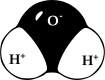
\includegraphics{content/introduction/graphics/polarWater}
        \end{center}
        \caption{Molecular model of a water molecule}
        \label{fig:waterMolecule}
    \end{figure}

    Water is a liquid comprised of the molecule $H_{2}O$.
    A molecular diagram of water is shown in figure~\ref{fig:waterMolecule}.
    This molecule is polar, meaning one side has a net positive charge and the other has a net negative charge.
    This imbalance is responsible for very complex behaviour when dealing with a liquid body of any reasonable size.
    Water molecules can rotate and migrate so as to neutralise an electrical field.
    This means that a body of water, or any polar liquid, behaves as an extremely lossy transmission medium.
    In short, a body of water will do its best to counteract any electrical gradient it experiences.

    \begin{figure}[h]
        \begin{center}
            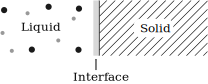
\includegraphics{content/introduction/graphics/simpleLayerDiagram}
        \end{center}
        \caption{Diagram showing the location of the fluid-solid interface}
        \label{fig:interfaceDiagram}
    \end{figure}

    The boundary between any two states of matter is referred to as an interface.
    We are interested specifically in the dynamics of the solid-liquid interface.
    Figure \ref{fig:interfaceDiagram} shows the organisation of a solid-liquid interface.
    The interactions relevant to this thesis occur in a very thin layer on the liquid side of the interface.
    When there is a difference in charge between the solid surface and the liquid bulk, a double layer forms.

    The basic principle behind double layer formation is summarised in the following statements.
    Charge interacts with charge, whether as repulsion or attraction.
    The charge difference directly at the interface will be the largest, therefore any interactions will be strongest here.
    The charged elements in a solid are fixed in place, but in a liquid they are free to move.
    Because of this restriction, interactions must take place within the liquid phase.

    The term `solid' does not refer only to the walls of the container holding the liquid.
    It can also describe particles within the liquid itself.
    For example, milk for the most part is an emulsion of butterfat and water.
    This means that molecules of butterfat are dispersed throughout the milk.
    In this scenario the butterfat molecules can be considered as solids.
    A representation of a butterfat molecule is shown in figure~\ref{fig:butterfat}.
    Butterfat molecules stays dispersed because they are encapsulated by double layers.
    Each butterfat molecule is electrically shielded from others around it by the double layer surrounding it.
    Without the layer the butterfat molecules will coagulate and the milk will turn lumpy.

    \begin{figure}
        \begin{center}
            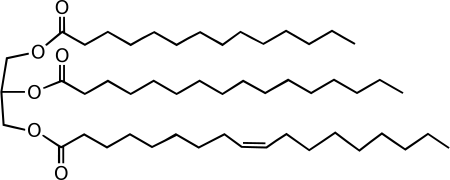
\includegraphics[scale=0.8]{content/introduction/graphics/butterfat}
        \end{center}
        \caption{Structural formula of a butterfat molecule}
        \label{fig:butterfat}
    \end{figure}

    We now know where double layers form, that they are organised states of liquid, and the kinds of behaviour they are responsible for.
    Next, we look at the anatomy of a double layer look at some of its properties.

  \subsection{The interfacial double layer}

    In the previous section we discussed where and why double layers form, but we haven't yet addressed what they are.
    We now look into double layers themselves and define some of their properties.

  \subsubsection*{Models of the interfacial double layer}
    \begin{figure}
      \begin{center}
        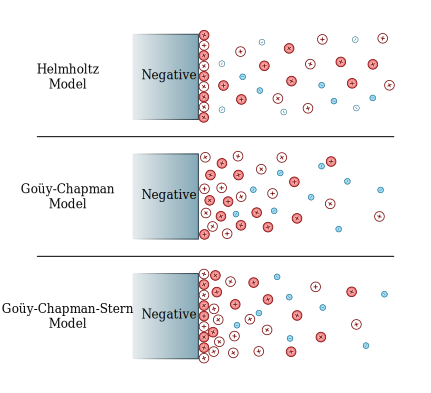
\includegraphics{content/introduction/graphics/doubleLayerModels}
      \end{center}
      \caption{Three models of double layer anatomy}
      \label{fig:doubleLayerModels}
    \end{figure}
  
    There are three models for the interfacial double layer.
    The general schematic behind each model is shown in figure~\ref{fig:doubleLayerModels}.
    Note that the solid need not be negatively charged.
    Each model is a progression of the previous model beginning with the Helmholtz model~\cite{Horch2004}.

    The first was proposed by Helmholtz in 1879 as a simple parallel plate capacitor model~\cite{Geddes1997}.
    This is represented by two layers of charge, one inside the solid and one in the liquid.
    Referring to figure~\ref{fig:doubleLayerModels}, this equates to a layer of electrons at solid surface matched by an immobile layer of positive ions at the liquid surface.
    Past the layer of bound surface ions there is no affect from the solids surface charge.

    The second model



    

  \subsubsection*{Anatomy of an interfacial double layer}

    \begin{figure}
      \begin{center}
        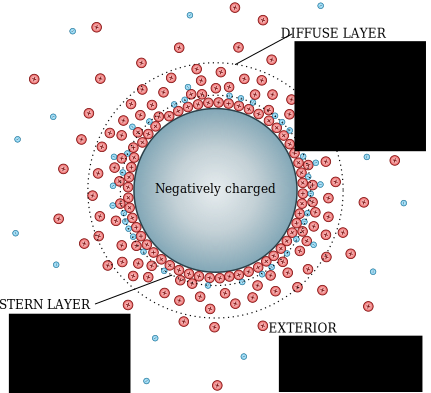
\includegraphics{content/introduction/graphics/doubleLayer_labelled.pdf}
      \end{center}
      \caption{Anatomy of the double layer}
      \label{fig:doubleLayer_anatomy}
    \end{figure}

    Figure~\ref{fig:doubleLayer_anatomy} shows the generic layout of a double layer.
    Owing to its name, it is broken into two distinct layers; the Stern and diffuse layers.
    The Stern layer is a compact layer of ions and molecules that are bound so tightly to the surface that they are immobile.
    This layer is typically in the order of one to ten 

    Double layer formation is the result of a liquid system responding to an imbalance of charge distribution.
		Atoms within a solid domain are static, they cannot repel each other or rearrange themselves.
		In a fluid the opposite is true, each freely moving charged entity will attempt to distance itself from others of like charge and move toward those of opposite charge.
		When these two domains are brought into contact with one another, the one whose elements are free to move (the liquid), moves to accommodate the imbalance in charge between the two domains.
		The effect of which is that an electrolytic liquid attracts atoms and molecules with a net opposite charge to the surface of the solid.

  \subsubsection*{Formation}
    {\color{blue}
    In order for a double layer to form, the liquid phase must contain ions, charged molecules, or polar molecules.
    This means there are likely to be non-participating elements within the fluid, that is, elements not affected by the charge {Todo: check affected and effected} of surrounding elements.
    The reverse case is also true {Todo: is this correct?, I just made it up} where an electrolyte solution comes in contact with a electrically neutral and stable solid.
		Although this case is not as obvious as one may think.
		For example, placing pure water in a glass flask, it may be assumed, would not cause the formation of a double layer.
		Glassware in used throughout chemistry laboratories as it reacts with very little and pure water with no salt ions should be fairly stable.
		This is not the case however as glass in contact with water undergoes a process of deprotonation at the boundary.
		This deprotonation is where $H^{+}$ ions are torn from the surface of the glass and enter the liquid phase.
		As this happens, the surface of the glass is left negatively charged.
		Subsequently, a double layer is formed from polar water molecules and hydrated protons.
    }



    Figures \ref{fig:doubleLayer_set1} and \ref{fig:doubleLayer_set2} illustrate the formation of such a layer around a charged object that, for the sake of illustration, instantaneously appears in a settled electrolyte solution.
		In these figures, the spacing of depicted fluid elements do not represent the density of a liquid system and the smooth surface of the charged object in no way resembles the surface of a solid at the scale of individual atoms.

    The first set of images, figure \ref{fig:doubleLayer_set1}, depict charged elements in the fluid responding to the presence of the solid by aligning themselves with the induced field and migrating toward or away from the object.
		The second set of images, figure \ref{fig:doubleLayer_set2}, shows continued migration of charged particles and the formation of the Stern layer at the solid-liquid interface.
		Members of this layer are bound so strongly to the object that they are effectively immobile, i.e., they are adsorbed to the solid object.
		A substantial proportion of the initial electrical field from the solid is shielded by the Stern layer.

    Outside the Stern layer, as the field strength continues to diminish with increasing radial distance, ions and molecules are attracted with decreasing strength.
		This reduction in attraction forms a layer that is thicker than the stern layer and mobile; the ions are free to move locally within this secondary layer.
		This secondary layer is called the diffuse layer and it is convenient to visualise it as a fluffy cloud of charged particles attracted to, but not trapped upon, the thin Stern layer immediately adjacent to the surface.

    \begin{figure}
      \begin{center}
        \includegraphics{content/introduction/graphics/doubleLayer_t0.pdf}
        \includegraphics{content/introduction/graphics/doubleLayer_t1.pdf}
        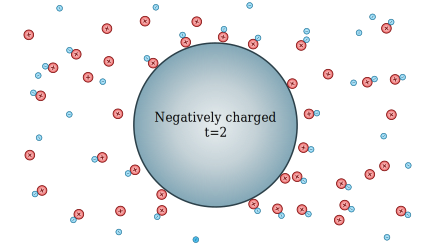
\includegraphics{content/introduction/graphics/doubleLayer_t2.pdf}
      \end{center}
      \caption{Creation of a double layer (time 0-2)}
      \label{fig:doubleLayer_set1}
    \end{figure}

    \begin{figure}
      \begin{center}
        \includegraphics{content/introduction/graphics/doubleLayer_t3.pdf}
        \includegraphics{content/introduction/graphics/doubleLayer_t4.pdf}
        %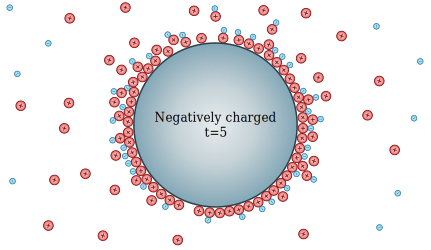
\includegraphics{content/introduction/graphics/doubleLayer_t5.pdf}
        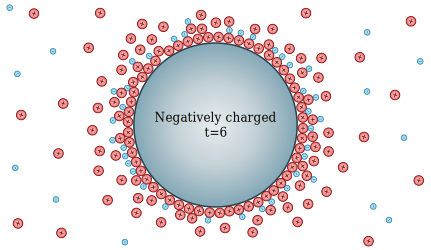
\includegraphics{content/introduction/graphics/doubleLayer_t6.pdf}
      \end{center}
      \caption{Creation of a double layer (time 3-6)}
      \label{fig:doubleLayer_set2}
    \end{figure}


  \subsection{Liquid simulation}
    \label{sub:molecularSimulation}

    At the macroscopic scale, liquid behaviour is simple and calculable.
    Modern computers can simulate the movement of liquids using the Navier-Stokes equations with accuracy and speed.
    Engineers simulate the flow of liquids, or any Newtonian fluid, routinely using computer design tools.
    These tools allow engineers to push boundaries of aircraft and boat design.
    This does not hold true when modelling fluid at the microscopic scale.

    Computer simulations usually involve calculating the state of a system of objects at specific time intervals.
    The process is repeated at each time step until the simulation time frame has been completed.
    These simulations are not run in real-time.
    In some cases they may take hours or days to complete a simulation spanning fractions of a second.

    Finite-difference time-domain simulation is a common technique for calculating electrical fields and resulting currents and voltages in the field of electrical engineering.
    Such simulations can involve hundreds of thousands, \emph{sometimes millions}, of objects.
    These objects are elements of a 3D mesh created to represent the geometry of the system.
    In such a simulation, each mesh element at every time step needs its various parameters (e.g. temperature, electromagnetic fields, electrical current and voltage) to be calculated based on the parameters of neighbouring objects in the mesh.
    Because of the dependence on neighbouring parameter values, each time-step may take many passes over each element in a system to calculate the final state before moving on.
    This type of simulation is common whenever the effects of radio waves need to be simulated.

    It seems natural to assume that molecular simulation of an interface would prove helpful.
    Doing so would allow simulation of the interactions taking place at the solid-fluid interface.
    Firstly, running molecular simulations requires knowing what species are present in the liquid and their relative abundances.
    This will not always be the case, especially in the human body or in tap water.
    Secondly, simulation of a body of liquid having a sensible volume is impractical.

    {\color{blue} Edited to here

    Say people don't know exactly whats happening at the double layer.
    Read some papers about molecular simulation
    }

    The molar mass of water is \SI{18.0528}{\gram\per\mole}, which represents the amount of water in moles per gram. 
    One gram of water is defined as one millilitre so we can say that for every millilitre of water we have we have an eighteenth of a mole of water. 
    Avagadro's constant, the number of constituent particles per mole of a given substance, is $6.0221\thinspace \times 10^{23}$.
    Therefore we have one eighteenth of Avagadro's constant in water molecules, which is about $3.3333\times 10^{22}$ molecules.
    That is 33 333 333 333 333 333 333 333 molecules!
    Relevant simulations are likely to require volumes greater than \SI{1}{\milli\litre} to be useful.
    
    Molecular simulation has not been employed in this work.
    There may be ways of simplifying necessary simulations in order to grain results from reduced systems.
    Molecular simulation is a very interesting


  \subsubsection*{Electrical Behaviour}

\section{Motivation}
  This thesis begins with the question: is it possible to harvest enough electrical energy from flowing water, without moving parts, to power a smart meter?
  The logic being that a harvester without moving parts would last longer than its mechanical equivalents.
  I started by investigating an assortment of possible mechanisms (discussed in detail in Chapter

  I started by investigating
  \begin{itemize}
    \item piezoelectric vibrators,
    \item electrostatic generators, and
    \item streaming potential cells
  \end{itemize}
  as potential harvesting mechanisims.

  The piezoelectric vibrator was the equivalent of a water whistle with a vibrational energy harvester attached.
  The electrostatic generator was a version of Lord Kelvin's Electrostatic Generator with a harvesting application.
  The streaming potential cell was a mystery.

  We knew geologists used streaming potentials to measure underground water flow.
  All we knew about the mechanism was that forcing water through something generated a voltage somehow.
  It was learning about that mechanism and answering the following questions that started me on what became this thesis.
  \begin{enumerate}
    \item Where does the streaming voltage come from?
    \item What role does the geometry of the device play?
    \item Could you change the materials to get more voltage?
  \end{enumerate}
  I eventually concluded that streaming cell harvesters were not practical for our application.
  By this time I had a working knowledge of interfacial double layers and their properties.

  My supervisor, Jonathan Scott, was on a sabbatical at Saluda Medical working with implant electrodes.
  There he developed an electrical model of the impedance presented by electrodes immersed in a solution of saline.
  This model would predict the electrical impedance seen between two electrodes when implanted in the spine of a human.
  Most of the behaviour the model reproduced was a result of interfacial double layers.

  Saluda wanted to know how good a substitute saline was for spinal fluid with regards to electrical impedance.
  There was no way to know and no way to compare solutions, except for using the new model.
  I took the model and started the next stage of my research; characterising fluids based on the impedance they present to electrodes.
  I was able to leverage my understanding of interfacial double layers and apply it to medical engineering.

\section{Publications}

\section{Thesis Outline}
